\documentclass{beamer}
\usetheme[block=fill]{metropolis}
\usepackage{graphicx}
\graphicspath{{../../latex/images/}}
\usepackage{boolexpr}
\usepackage{kpfonts}
\usepackage{caption}
\usepackage{wrapfig}
\usepackage[labelformat=empty]{caption}
\usepackage[official]{eurosym}

\usepackage{animate}

\usepackage[charsperline=60]{jlcode}
\addlitjlmacros{@constraint}{@constraint}{11}
\addlitjlmacros{@variable}{@variable}{9}
\addlitjlmacros{@objective}{@objective}{10}


\usepackage{siunitx}

\usepackage[math]{iwona}
\usepackage{scalerel}
\def\lVert{\mid\!\mid}
\def\rVert{\mid\!\mid}

\usepackage[normalem]{ulem}
\usepackage{mathtools}

\usepackage{../../latex/custom}
\usepackage{amsfonts}

\usepackage{tikz}
\usetikzlibrary{arrows,matrix,decorations.pathreplacing,positioning,chains,fit,shapes,calc,3d}
\tikzset{box/.style={rectangle, draw=black, fill=black!8, align=center, rounded corners}}
\tikzset{rep/.style={rectangle, draw=julia_blue, fill=julia_blue!8, align=center, rounded corners}}

\definecolor{julia_blue}{rgb}{0.251, 0.388, 0.847}
\definecolor{julia_green}{rgb}{0.22 , 0.596, 0.149}
\definecolor{julia_purple}{rgb}{0.584, 0.345, 0.698}
\definecolor{julia_red}{rgb}{0.796, 0.235, 0.2  }

\newcommand{\expe}[2]{\la #1, #2 \ra}

\usepackage{framed}

\newcommand\Wider[2][3em]{%
\makebox[\linewidth][c]{%
  \begin{minipage}{\dimexpr\textwidth+#1\relax}
  \raggedright#2
  \end{minipage}%
  }%
}

\newcommand{\aeur}{\alpha_\text{\euro}}
\newcommand{\adol}{\alpha_\$}
\newcommand{\apou}{\alpha_\text{\pounds}}

\title{Polyhedral Computation }
\date{July 26th, 2023}
\author{Beno\^it Legat}
\institute{
  \begin{minipage}{\textwidth}
    ERC ``Back to the Roots'' with Prof. Bart De Moor, STADIUS, KU Leuven

    \vspace{4em}
    
    \hfill
\includegraphics[width=0.15\textwidth]{JuliaCon.png}
  \end{minipage}
}

\makeatletter
\let\@@magyar@captionfix\relax
\makeatother
\begin{document}
  \maketitle

  \begin{frame}
    \frametitle{What is Polyhedral Computation}
    \begin{center}
      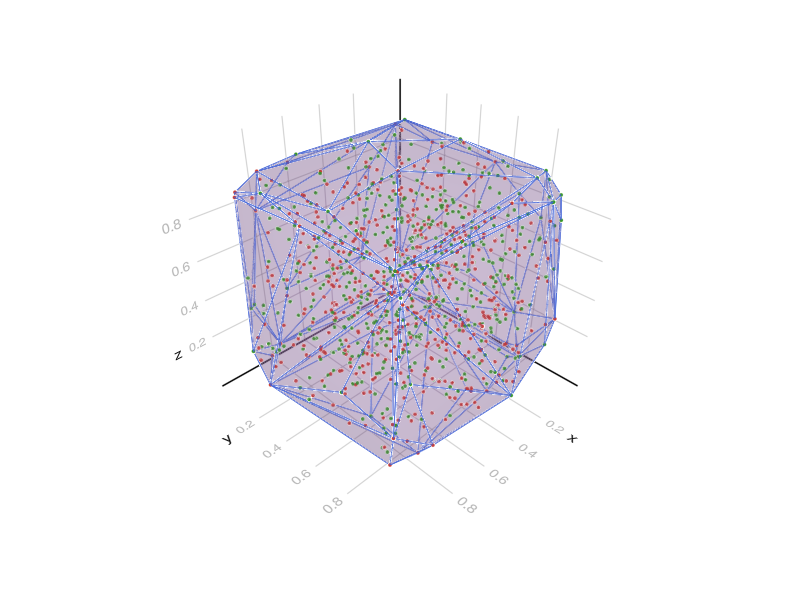
\includegraphics[width=\textwidth]{vpolyhedra_julia.png}
    \end{center}
  \end{frame}

  \begin{frame}
    \frametitle{What is it used for ?}
    \begin{columns}
      \begin{column}{0.45\textwidth}
        \begin{block}{Reachability analysis}
          \begin{center}

            \vspace{-1em}

            
\includegraphics[width=0.6\textwidth]{Dionysos.png}~%

            \vspace{-1em}

            
\includegraphics[width=0.4\textwidth]{juliareach.png}~%
            \raisebox{1.7em}{JuliaReach} %

            \vspace{-1.2em}
          \end{center}
        \end{block}
        \begin{block}{Invariant sets}
          \begin{center}
            \scriptsize
            \vspace{-0.5em}

            \jlpkg{InvariantSets}


            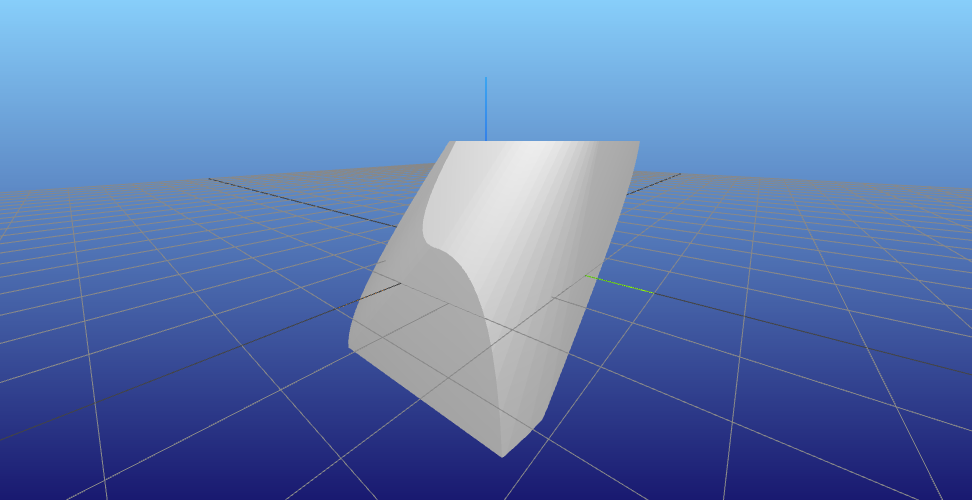
\includegraphics[width=0.4\textwidth]{tow/0000006.png}

            \vspace{-0.6em}

            \jlpkg{SetProg}, \jlpkg{SwitchOnSafety}

            \vspace{-0.8em}


            
\includegraphics[width=0.33\textwidth]{tetra0zy.png}~%
            
\includegraphics[width=0.33\textwidth]{tetra1bound1585.png}

            \vspace{-0.8em}

            \jlpkg{EntropicCone}

            \vspace{-0.4em}
          \end{center}
        \end{block}
      \end{column}
      \begin{column}{0.45\textwidth}
        \begin{block}{Delaunay tesselation}

            \scriptsize
          \jlpkg{HyperVoronoiDelaunay}, \jlpkg{VoronoiGraph}, \jlpkg{LaguerreVoronoi}, \jlpkg{VoroX}
        \end{block}
        \begin{block}{Game theory}
          \begin{center}
            \scriptsize
            \jlpkg{GameTheory}
          \end{center}
        \end{block}
        \begin{block}{Optimization}
          \begin{center}
            
\includegraphics[width=0.6\textwidth]{JuMP.png}
          \end{center}
        \end{block}
      \end{column}
    \end{columns}
  \end{frame}

  \begin{frame}
    \frametitle{Which libraries exists}
    \begin{columns}
      \begin{column}{0.45\textwidth}
        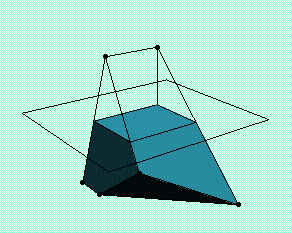
\includegraphics[width=0.4\textwidth]{cddlib.png}~
        \raisebox{2em}{\texttt{cddlib}}

        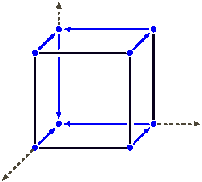
\includegraphics[width=0.4\textwidth]{lrslib.png}~
        \raisebox{2em}{\texttt{lrslib}}

        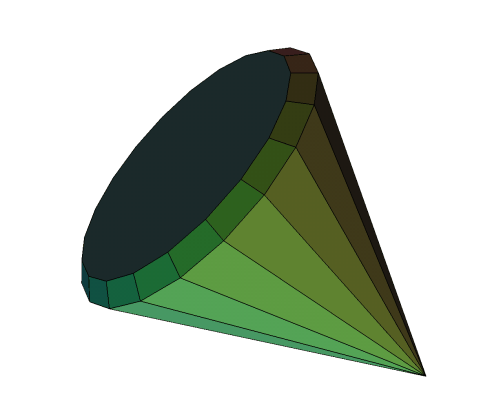
\includegraphics[width=0.4\textwidth]{qhull.png}~
        \raisebox{2em}{\texttt{qhull}}

        \begin{center}
        \texttt{pd}
        \end{center}
      \end{column}

      \begin{column}{0.45\textwidth}
        \begin{center}
        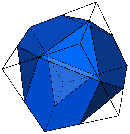
\includegraphics[width=0.3\textwidth]{porta.png}~
        \raisebox{1.8em}{\texttt{PORTA}}
        \end{center}


        \begin{center}
        
\includegraphics[width=0.3\textwidth]{ppl.png}

        \texttt{Parma Polyhedra Library (PPL)}
        \end{center}

        \begin{center}
        \jlpkg{ConvexHull}
        \end{center}
        \begin{center}
        \jlpkg{Polyhedra}
        \end{center}
      \end{column}
    \end{columns}
  \end{frame}

  \begin{frame}
    \frametitle{Fastest algorithm depend on the class of polyhedra}
    \Wider[2em]{
    \begin{columns}
      \begin{column}{0.33\textwidth}
        \begin{center}

        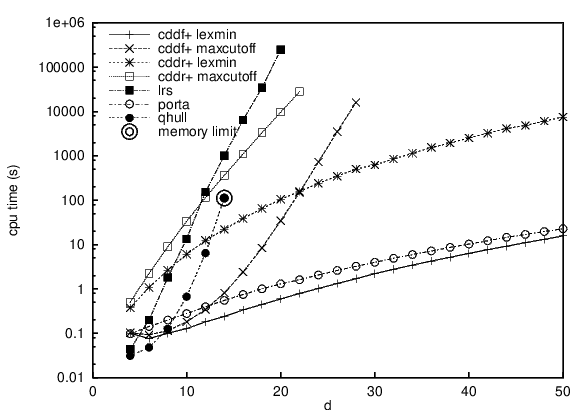
\includegraphics[width=1.0\textwidth]{cddwin.png}

        \footnotesize

        Double description

        \texttt{cddlib}, \texttt{porta}

        {\tiny
        \texttt{Rational\{BigInt\}} \texttt{cddr}
        \alert{faster} than \texttt{Float64} \texttt{qhull}}
        \end{center}
      \end{column}
      \begin{column}{0.33\textwidth}
        \begin{center}
        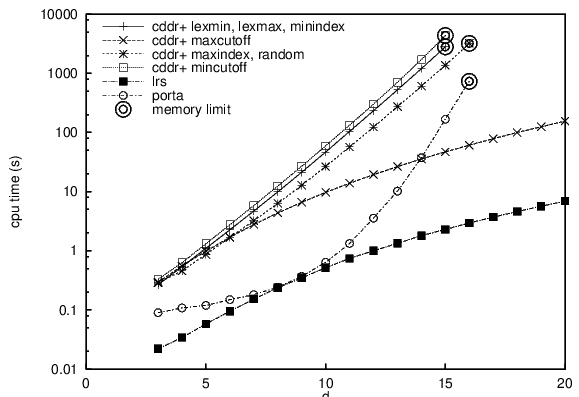
\includegraphics[width=1.0\textwidth]{lrswin.png}

        \footnotesize

        Reverse search
        
        \texttt{lrslib}

        {\tiny
        \texttt{Rational\{BigInt\}} \texttt{lrs}
        \alert{faster} than \texttt{Float64} \texttt{qhull}}
        \end{center}
      \end{column}
      \begin{column}{0.33\textwidth}
        \begin{center}
        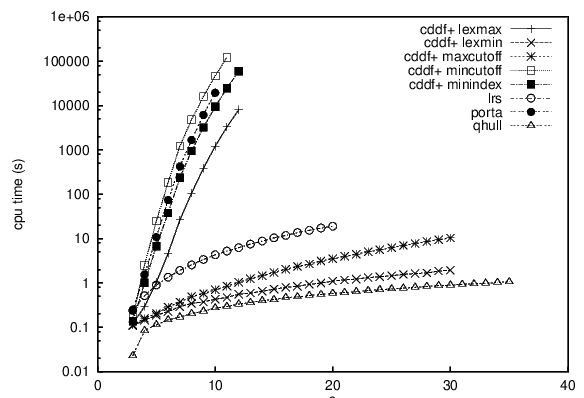
\includegraphics[width=1.0\textwidth]{qhullwin.png}

        Quick hull

        \texttt{qhull}

        {\tiny
        \texttt{Rational\{BigInt\}} \texttt{lrs}
        \alert{faster} than \texttt{Rational\{Int\}} \texttt{PORTA}}
        \end{center}
      \end{column}
    \end{columns}

    \vspace{2em}

    {
      \footnotesize
      Avis D, Bremner D.
      (1995)
      \emph{How good are convex hull algorithms?}\\
      Proceedings of the eleventh annual symposium on Computational geometry
    }

    \vspace{1em}

    \uncover<2>{
      {
        \footnotesize
        \jlpkg{InvariantSets} built on \jlpkg{Polyhedra} but alternatives have \alert{fixed} library
      }
    }
    }
  \end{frame}

\begin{frame}
    \frametitle{Just In Time representation conversion}
  \begin{center}
  \begin{tikzpicture}[scale = 1.2, every node/.style={scale=0.6}]
    \node[rep] (H)     at (-2,  0) {H-rep};
    \node[rep] (V)     at ( 2,  0) {V-rep};
    \node[box] (INT)   at (-4,  1) {$\cap$};
    \draw[thick, ->] (H.north west) to (INT.south east);
    \node[box] (CHEBY) at (-4, -1) {\begin{minipage}{3em}\centering Cheby center\end{minipage}};
    \draw[color=julia_purple, thick, ->] (H.south west) to node[rotate=20, below] {\includegraphics[width=4em]{jump.png}} (CHEBY.north east);
    \node[box] (CART)  at (-2.5,  2) {\begin{minipage}{4em}\centering Cartesian product\end{minipage}};
    \draw[color = julia_green, thick, ->] (H.north) to (CART.south);
    \draw[color = julia_red, thick, dashed, ->] (V.north west) to (CART.south east);
    \node[box] (PLOT)  at (-1,  2) {Plot};
    \draw[thick, -] (H.north east) to (-1, 1);
    \draw[thick, -] (V.north west) to (-1, 1);
    \draw[thick, ->] (-1, 1) to (PLOT.south);
    \node[box] (VOL)   at ( 1,  2) {Volume};
    \draw[thick, -] (H.north east) to ( 1, 1);
    \draw[thick, -] (V.north west) to ( 1, 1);
    \draw[thick, ->] ( 1, 1) to (VOL.south);
    \node[box] (IN)    at (2.5,  2) {\texttt{in}};
    \draw[color=julia_green, thick, ->] (H.north east) to (IN.south west);
    \draw[color=julia_red, thick, -] (V.north) to (IN.south);
    \draw[color=julia_purple, thick, dashed, ->] (V.north) to node[rotate=75, below] {\includegraphics[width=4em]{jump.png}} (IN.south);
    \node[box] (PLUS)  at ( 4,  1) {$+$};
    \draw[dashed, thick, ->] (V.north east) to (PLUS.south west);
    \node[box] (CONVH) at ( 4, -1) {Convex hull};
    \draw[thick, ->] (V.south east) to (CONVH.north west);
    \node[box] (AM)    at ( 2, -2) {$A \times \cdot$};
    \draw[thick, ->] (V.south) to (AM.north);
    \node[box] (AB)    at (-2, -2) {$A \backslash \cdot$};
    \draw[thick, ->] (H.south) to (AB.north);
    \node[box] (PROJ)  at ( 0, -2) {Project};
    \draw[color = julia_red, thick, dashed, ->] (H.south east) to (PROJ.north west);
    \draw[color = julia_green, thick, ->] (V.south west) to (PROJ.north east);
    \node[box] (TR)    at ( 0,  0) {Translate};
    \draw[thick, ->] (H.east) to (TR.west);
    \draw[thick, ->] (V.west) to (TR.east);

    \draw[color = julia_green, thick, ->]  (-4, -2.5) to (-3.5, -2.5) node[right] {Preferred};
    \draw[color = julia_red, thick, ->]    (-4, -2.8) to (-3.5, -2.8) node[right] {Fallback if other rep not computed};
    \draw[color = julia_purple, thick, ->] (-4, -3.1) to (-3.5, -3.1) node[right] {Solve linear program using \includegraphics[height=1em]{jump.png}};
    \draw[dashed, thick, ->]               (-4, -3.4) to (-3.5, -3.4) node[right] {Size of resulting representation may grow significantly};
  \end{tikzpicture}
  \end{center}
\end{frame}


  \begin{frame}
    \frametitle{\jlpkg{Polyhedra} interface}
    \begin{itemize}
      \item V-representation type
      \item H-representation type (can use \includegraphics[height=1em]{jump.png} model)
      \item Polyhedron type
      \begin{itemize}
        \item Detect redundancy and linearity (e.g. affine hull) with \includegraphics[height=1em]{jump.png}
        \item \alert{Transparently} H-convert or V-convert \alert{only} if needed
      \end{itemize}
      \item Interface implementation for libraries:
      \begin{itemize}
        \item Defaults to pure julia double description implementation
        \item \jlpkg{CDDLib} (\texttt{cddlib})
        \item \jlpkg{ConvexHull} by Joey Huchette
        \item \jlpkg{LRSLib} (\texttt{lrslib}) : Thanks Daisuke Oyama!
        \item \jlpkg{QHull} (\texttt{qhull}) : Thanks David van Leeuwen!
        \item \jlpkg{ParmaPolyhedra} (\texttt{PPL})
        \item \jlpkg{XPORTA} (\texttt{PORTA}) : Thanks Brian Doolittle!
      \end{itemize}
    \end{itemize}
  \end{frame}
\end{document}
